\documentclass[titlepaged,toc]{../cs-classes/cs-classes}

\title{Introduction to Robotics}
\author{Julien Carpentier\and Stéphane Caron\and Yann de Mont-Marin}

\begin{document}

\begin{abstract}
    This document is Antoine Groudiev's class notes while following the class \emph{Motion planning in robotics and graphical animation} (Planification de mouvement en robotique et en animation graphique) at the Computer Science Department of ENS Ulm. It is freely inspired by the lectures of Justin Carpentier, Stéphane Caron, and Yann de Mont-Marin.
\end{abstract}

\section{Introduction and general overview}
\subsection{What is Deep Learning?}
\subsubsection{Neural networks}
\subsubsection{Timeline of Deep Learning}
\subsubsection{Recent applications and breakthroughs}
\subsubsection{Usual setup}
\subsubsection{Required skills}
\subsubsection{Building blocks of deep learning}
\subsubsection{Why deep learning now?}

\subsection{Machine Learning pipeline}
\subsubsection{Cats vs. dogs}
\subsubsection{Typical Machine Learning setup}
\subsubsection{Training objective}

\subsection{Multi-Layer Perceptron}
\subsubsection{Definition}
\subsubsection{PyTorch implementation}
\section{Position and Orientation}
\subsection{Introduction}
Kinematics studies the \emph{movement} of an object -- in our case of a robot -- without taking into acount the \emph{forces} generating it. Instead, it only handles aspects such as position, orientation, speed and momentum of bodies in movement.

Consider for instance a robotic arm. We can design a simplified scheme of the robot and its environment, to create a kinematic pipeline and reference frames associated to each of these objects.

\begin{figure}[H]
    \centering
    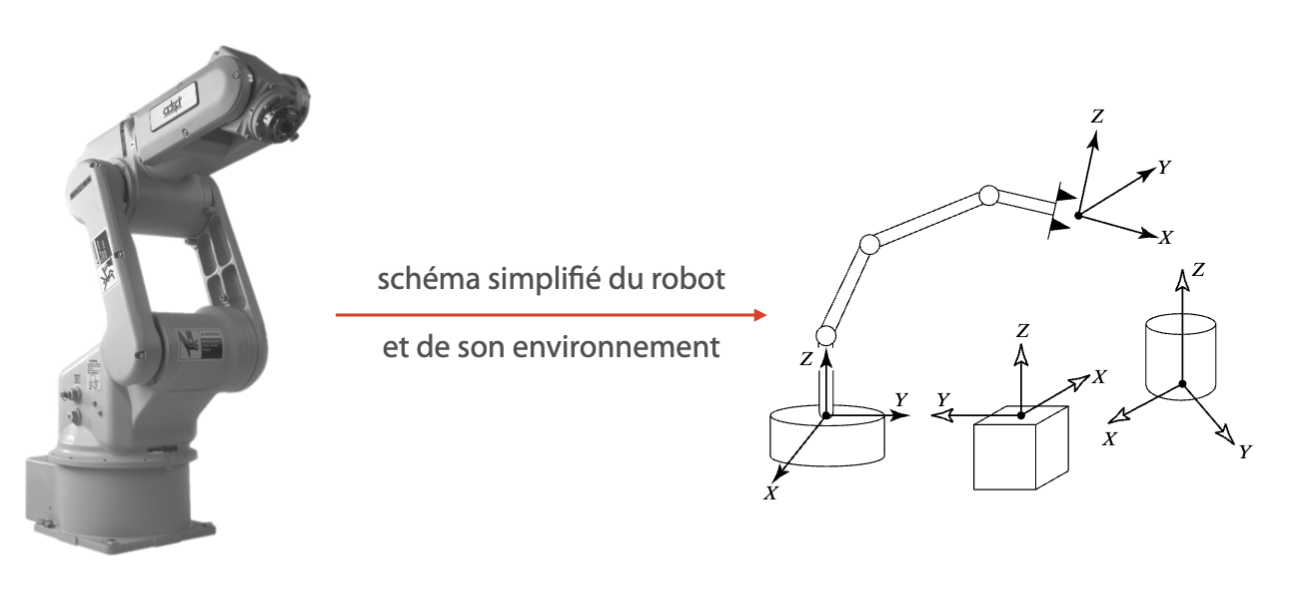
\includegraphics[width=.6\textwidth]{position/arm-scheme.png}
    \caption{Simplified scheme of the robot, the kinematic pipeline and reference frames.}
\end{figure}

\emph{Direct kinematics} allows to compute the position and orientation of the terminal organ given, for instance, the angles of the articulations.

\begin{figure}[H]
    \centering
    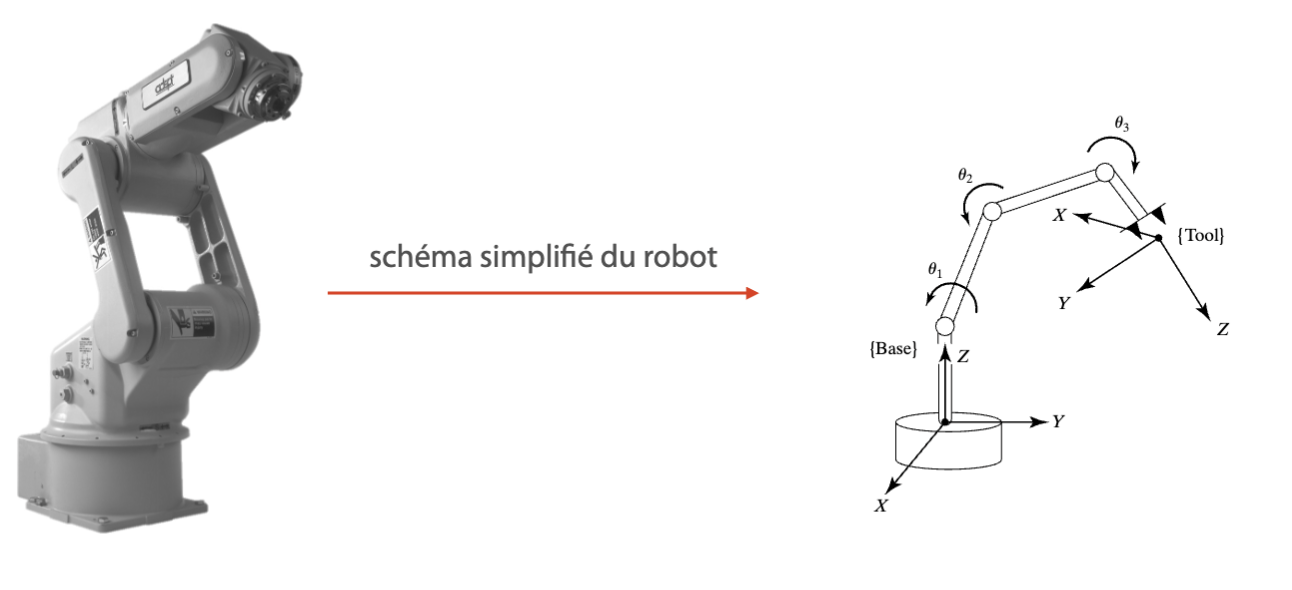
\includegraphics[width=.6\textwidth]{position/direct-kinematic.png}
\end{figure}

\emph{Invert kinematics} answers the question the other way around: given the position and orientation of a boyd, how can we compute the values of the articulations angles. Invert kinematics is used for instance for trajectory tracking: given a reference trajectory, how can we compute the speed of the articulations?

\subsection{Points, frames and transformations}
\subsubsection{Position of a point in space}
Once that a reference frame $\{A\}$ is defined, we can localize any point of the universe given a \emph{position vector}:
\begin{figure}[H]
    \centering

    \begin{minipage}{0.4\textwidth}
        \begin{equation*}
            \prescript{A}{}{P} = \begin{bmatrix}
                p_x \\ p_y \\ p_z
            \end{bmatrix}
        \end{equation*}
    \end{minipage}
    \begin{minipage}{0.4\textwidth}
        \centering
        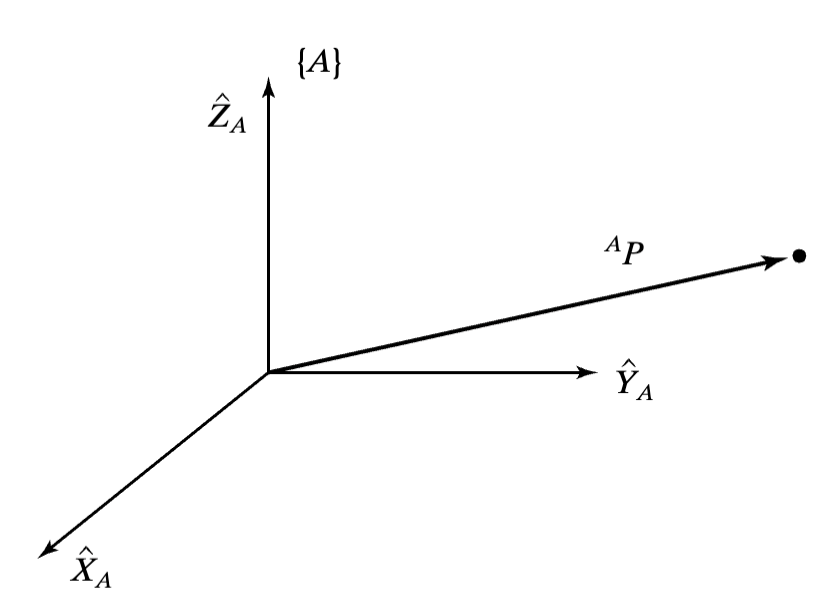
\includegraphics[width=.8\textwidth]{position/position-frame.png}
    \end{minipage}
    \caption{Vector and position of the point established in the frame $\{A\}$.}
\end{figure}

\subsubsection{Position and orientation of a body in space}
To define the orientation of a body in space, we need to define a reference frame $\{B\}$ attached to this body. The orientation is therefore defined as the expression of this coordinate system in the reference frame $\{A\}$.
\begin{figure}[H]
    \centering

    \begin{minipage}{0.5\textwidth}
        \begin{equation*}
            \prescript{A}{B}{R} = \begin{bmatrix}
                \prescript{A}{}{\hat{X}}_B & \prescript{A}{}{\hat{Y}}_B & \prescript{A}{}{\hat{Z}}_B
            \end{bmatrix}
            = \begin{bmatrix}
                r_{11} & r_{12} & r_{13} \\
                r_{21} & r_{22} & r_{23} \\
                r_{31} & r_{32} & r_{33}
            \end{bmatrix}
        \end{equation*}
    \end{minipage}
    \begin{minipage}{0.4\textwidth}
        \centering
        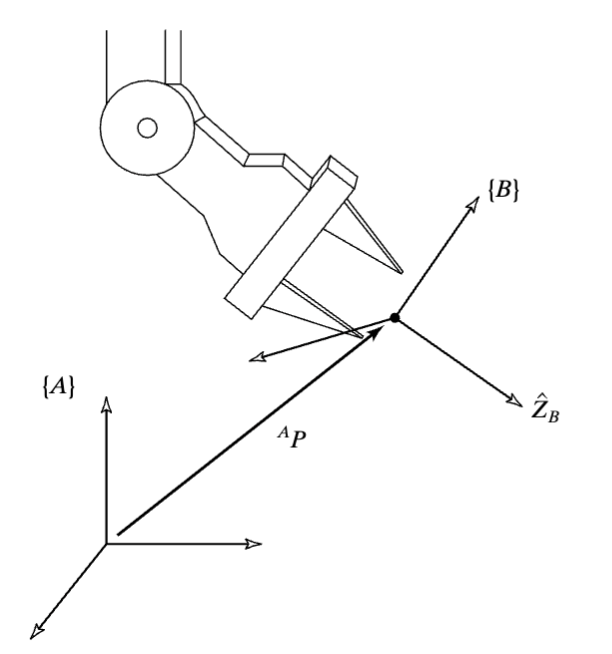
\includegraphics[width=.8\textwidth]{position/body-orientation.png}
    \end{minipage}
    \caption{Expression of the coordinate system $\{B\}$ in the reference frame $\{A\}$, and the associated position and orientation of the body.}
\end{figure}
Each element of the matrix $\prescript{A}{B}{R}$ is the scalar product between the vectors of the two coordinate systems $\{B\}$ and $\{A\}$:
\begin{equation*}
    \prescript{A}{B}{R} = \begin{bmatrix}
        \prescript{A}{}{\hat{X}}_B & \prescript{A}{}{\hat{Y}}_B & \prescript{A}{}{\hat{Z}}_B
    \end{bmatrix}
    = \begin{bmatrix}
        \hat{X}_B\cdot\hat{X}_A & \hat{Y}_B\cdot\hat{X}_A & \hat{Z}_B\cdot\hat{X}_A \\
        \hat{X}_B\cdot\hat{Y}_A & \hat{Y}_B\cdot\hat{Y}_A & \hat{Z}_B\cdot\hat{Y}_A \\
        \hat{X}_B\cdot\hat{Z}_A & \hat{Y}_B\cdot\hat{Z}_A & \hat{Z}_B\cdot\hat{Z}_A
    \end{bmatrix}
\end{equation*}
The lines correspond to the axes of the frame $\{A\}$ expressed in the frame $\{B\}$. Note that the invert of a rotation matrix is its transpose:
\begin{equation*}
    \prescript{A}{B}{R}^T = \prescript{A}{B}{R}^{-1} = \prescript{B}{A}{R}
\end{equation*}

\subsubsection{Rotation matrices}
We showed that the orientation of the body in space could be expressed as a 3-dimensional rotation matrix. The group of 3-dimensional rotation matrices is denoted $\SO(3)$, and is composed of all the matrices that are orthonormal, that is orthogonal and with a determinant equal to 1:
\begin{equation}
    \SO(3) = \set{R\in\mathcal{M}_{3}(\R)}{RR^T=I_3 \text{ and } \det(R) = +1}
\end{equation}
If we write:
\begin{equation*}
    R = \begin{bmatrix}
        \hat{X} & \hat{Y} & \hat{Z}
    \end{bmatrix}
\end{equation*}
Then $R\in\SO(3)$ if and only if:
\begin{equation*}
    \begin{cases}
        \hat{X}\cdot\hat{Y} = 0 \\
        \hat{Y}\cdot\hat{Z} = 0 \\
        \hat{Z}\cdot\hat{X} = 0 \\
    \end{cases}
    \quad\text{and}\quad
    \begin{cases}
        \hat{X}\cdot\hat{X} = 1 \\
        \hat{Y}\cdot\hat{Y} = 1 \\
        \hat{Z}\cdot\hat{Z} = 1 \\
    \end{cases}
\end{equation*}
Note that we have 9 degrees of freedom and 6 independent constraints, so the group $\SO(3)$ is 3-dimensional.

\subsection{Rotation representations}
There are several ways to represent a rotation matrix, each with its own advantages and drawbacks. The most common representations are:
\begin{itemize}
    \item Orthonormal 3 by 3 matrices --- 9 components
    \item Euler angles --- 3 components
    \item Axis-angle representation --- 3 components
    \item Quaternions --- 4 components
\end{itemize}
The number of components used to be an important factor when computers were slow and memory was expensive. Nowadays, the choice of representation is more about the ease of use and the properties of the representation.

\subsubsection{Euler angles}
Each rotation can be represented by the composition of three elementary rotations around the fixed axes of the frame $\{A\}$.
\begin{figure}[H]
    \centering
    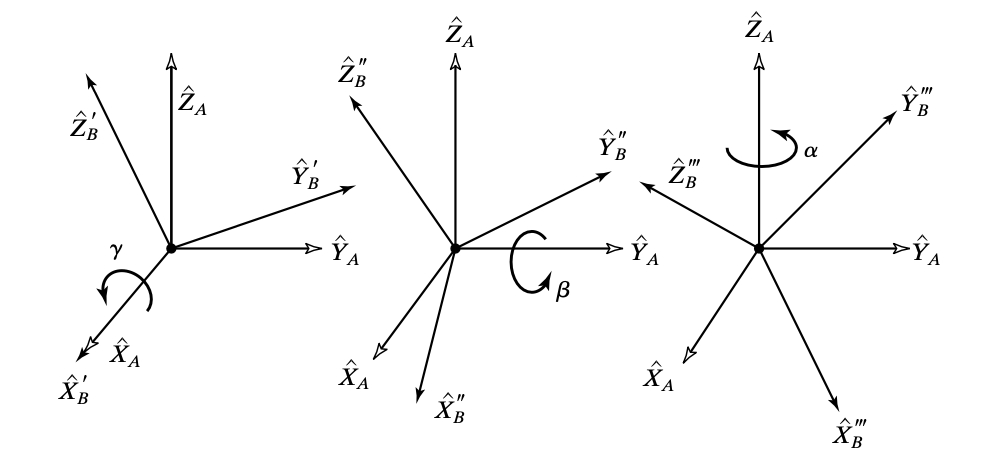
\includegraphics[width=.6\textwidth]{position/euler-angles.png}
    \caption{Euler angles representation of a rotation.}
\end{figure}
In terms of rotation matrices, any rotation matrix can be written as $\prescript{A}{B}{R}(\gamma, \beta, \alpha)$, defined by:
\begin{align*}
    \prescript{A}{B}{R}(\gamma, \beta, \alpha) &= R_Z(\alpha)R_Y(\beta)R_X(\gamma)\\
    &= \begin{bmatrix}
        \cos\alpha & -\sin\alpha & 0 \\
        \sin\alpha & \cos\alpha & 0 \\
        0 & 0 & 1
    \end{bmatrix}
    \begin{bmatrix}
        \cos\beta & 0 & \sin\beta \\
        0 & 1 & 0 \\
        -\sin\beta & 0 & \cos\beta
    \end{bmatrix}
    \begin{bmatrix}
        1 & 0 & 0 \\
        0 & \cos\gamma & -\sin\gamma \\
        0 & \sin\gamma & \cos\gamma
    \end{bmatrix}
\end{align*}
The Euler angles are not unique, as the same rotation can be represented by different sets of Euler angles. This is called gimbal lock, and is a major drawback of the Euler angles representation.

We can also express the Euler angles given the rotation matrix:
\begin{align*}
    \prescript{A}{B}{R}(\gamma, \beta, \alpha) = \begin{bmatrix}
        r_{11} & r_{12} & r_{13} \\
        r_{21} & r_{22} & r_{23} \\
        r_{31} & r_{32} & r_{33}
    \end{bmatrix}
    \implies
    \begin{cases}
        \beta = \atantwo(-r_{31}, \sqrt{r_{11}^2+r_{21}^2}) \\
        \alpha = \atantwo(r_{21}/\cos\beta, r_{11}/\cos\beta) \\
        \gamma = \atantwo(r_{32}/\cos\beta, r_{33}/\cos\beta)
    \end{cases}
\end{align*}

\subsubsection{Axis-angle and quaternions}
We are given a vector $\vec{k}$ and an angle $\theta$; the rotation represented by these two elements is the rotation of angle $\theta$ around the axis $\vec{k}$. We can define:
\begin{equation*}
    \begin{cases}
        \epsilon_1 = k_x\sin\frac{\theta}{2} \\
        \epsilon_2 = k_y\sin\frac{\theta}{2} \\
        \epsilon_3 = k_z\sin\frac{\theta}{2} \\
        \epsilon_4 = \cos\frac{\theta}{2}
    \end{cases}
\end{equation*}
we have $\epsilon_1^2+\epsilon_2^2+\epsilon_3^2+\epsilon_4^2=1$, creating a unit quaternion. The rotation matrix associated to the quaternion is:
\begin{equation*}
    R_\epsilon = \begin{bmatrix}
        1-2\epsilon_2^2-2\epsilon_3^2 & 2(\epsilon_1\epsilon_2-\epsilon_3\epsilon_4) & 2(\epsilon_1\epsilon_3+\epsilon_2\epsilon_4) \\
        2(\epsilon_1\epsilon_2+\epsilon_3\epsilon_4) & 1-2\epsilon_1^2-2\epsilon_3^2 & 2(\epsilon_2\epsilon_3-\epsilon_1\epsilon_4) \\
        2(\epsilon_1\epsilon_3-\epsilon_2\epsilon_4) & 2(\epsilon_2\epsilon_3+\epsilon_1\epsilon_4) & 1-2\epsilon_1^2-2\epsilon_2^2
    \end{bmatrix}
\end{equation*}

The invert operation is also simple to compute:
\begin{align*}
    \prescript{A}{B}{R}(\gamma, \beta, \alpha) = \begin{bmatrix}
        r_{11} & r_{12} & r_{13} \\
        r_{21} & r_{22} & r_{23} \\
        r_{31} & r_{32} & r_{33}
    \end{bmatrix}
    \implies
    \begin{cases}
        \epsilon_1 = \frac{r_{32}-r_{23}}{4\epsilon_4} \\
        \epsilon_2 = \frac{r_{13}-r_{31}}{4\epsilon_4} \\
        \epsilon_3 = \frac{r_{21}-r_{12}}{4\epsilon_4} \\
        \epsilon_4 = \frac{1}{2}\sqrt{1+r_{11}+r_{22}+r_{33}}
    \end{cases}
\end{align*}

\subsection{Angular velocity}
The angular velocity of a body is a vector that describes the rotation of the body in space. It is defined as the derivative of the rotation matrix with respect to time. Angular velocity matrices are skew-symmetric matrices, i.e. matrices of the tangent space of $\SO(3)$, denoted $\so(3)$:
\begin{equation*}
    \so(3) = \set{W\in\mathcal{M}_3(\R)}{W^\tp=-W} = \set{\begin{bmatrix}
        0 & -w_z & w_y \\
        w_z & 0 & -w_x \\
        -w_y & w_x & 0
    \end{bmatrix}}{w_x, w_y, w_z\in\R}
\end{equation*}
Indeed, consider the rotation matrix $R(t)\in\SO(3)$, and denote $\dot R(t) = \partfrac{R(t)}{t}$ the derivative of $R(t)$ with respect to time. We have:
\begin{align*}
    R(t)R(t)^\tp &= I_3 \\
    \dot RR^\tp + R\dot R^\tp &= 0_3 \\
    \dot RR^\tp &= -R\dot R^\tp \\
    \dot RR^\tp &= -\left(\dot RR^\tp\right)^\tp \\
\end{align*}
Hence, by defining $W := \dot RR^\tp$, we have $W\in\so(3)$.

Note that $R(t)$ is the solution of the differential equation $\dot R = WR$, with $R(0)=R_0\in\SO(3)$. The solution is:
\begin{equation*}
    R(t) = R_0\exp(Wt) \quad\text{where}\quad \exp(Wt) = \sum_{n=0}^{+\infty}\frac{(Wt)^n}{n!}
\end{equation*}
This gives us a new parameterization of the group $\SO(3)$, using the angular velocity matrices. Recall that a matrix $W\in\so(3)$ is associated to a vector $w=(w_x, w_y, w_z)\in\R^3$; we denote $\hat{w}=W$. The main question associated to this representation is to compute the infinite sum of the exponential function:
\begin{equation}
    \exp(tW)=\sum_{n=0}^{+\infty}\frac{(tW)^n}{n!}
\end{equation}
We can use the fact that any skew-symmetric matrix $W\in\so(3)$ is nilpotent, i.e. there exists an integer $n\in\N$ such that $W^n=0_3$. This allows us to compute the exponential function:
\begin{equation*}
    \hat{w}=W=\begin{bmatrix}
        0 & -w_z & w_y \\
        w_z & 0 & -w_x \\
        -w_y & w_x & 0
    \end{bmatrix} = w \times \cdot
\end{equation*}
Therefore, $\hat{w}^2=ww^\tp-I_3$, and $\hat{w}^3=-\hat{w}$. We can then regroup the different terms of the exponential function, by transforming the exponents greater than 3:
% TODO: detail computation
\begin{equation}
    \exp(tW)=I_3+\sin(t)\hat{w}+\frac{1-\cos(t)}{t}\hat{w}^2
\end{equation}

\subsection{Exponential and logarithm map}
We saw that the exponential map is an application from the tangent space of $\SO(3)$, $\so(3)$ to the group $\SO(3)$, defined by:
\begin{align*}
    \exp:\so(3)&\longrightarrow\SO(3)\\
    tW&\longmapsto\exp(tW) = I_3 + \sin(t)\hat{w} + \frac{1-\cos(t)}{t}\hat{w}^2
\end{align*}
This function is surjective and $2\pi$-periodic.

We can define a reciprocal function, the logarithm map, that is the inverse of the exponential map:
\begin{equation*}
    \log:R\in\SO(3)\longrightarrow w\in\so(3)
\end{equation*}
Note that
\begin{equation*}
    \norm{w}=\cos^{-1}\left(\frac{\Tr(R)-1}{2}\right)
\end{equation*}
and therefore:
\begin{equation*}
    w=\frac{\norm{w}}{2\sin(\norm{w})}\begin{bmatrix}
        r_{32}-r_{23} \\
        r_{13}-r_{31} \\
        r_{21}-r_{12}
    \end{bmatrix}
\end{equation*}

This gives us a way to compute the distance between two rotations:
\begin{equation*}
    d(R_1, R_2) = \norm{\log(R_1^\tp R_2)}
\end{equation*}
Such a construction comes handy when we want to minimize the distance between two rotations, for instance in the context of trajectory tracking.

\subsection{Rigid Body Transformations}

\section{Forward Kinematics}
\emph{Forward kinematics} allows to compute the position and orientation of the kinematic chain given the joint parameters (e.g. angles, lengths, etc.). For instance, we can compute the position and orientation of the terminal organ given the angles of the articulations.
\begin{figure}[H]
    \centering
    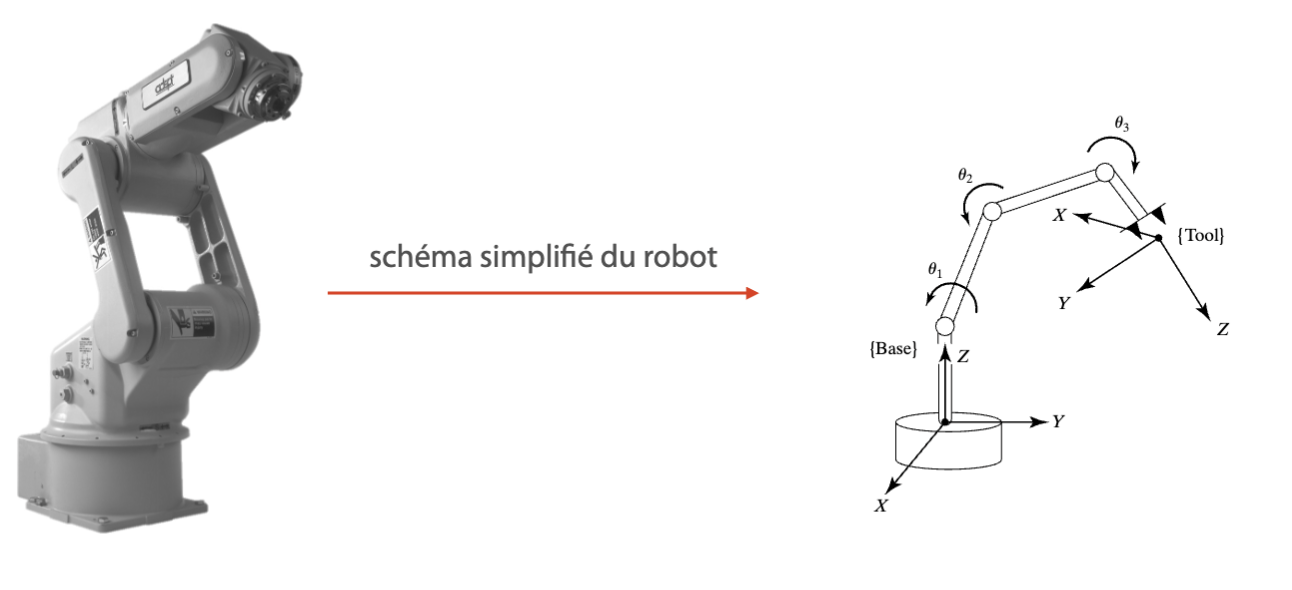
\includegraphics[width=.7\textwidth]{position/direct-kinematic.png}
\end{figure}

The kinematic chain is composed of rigid bodies interconnect by joints. The joins define the degrees of freedom of the cinematic chain, which are the parameters that we can control.
\begin{figure}[H]
    \centering
    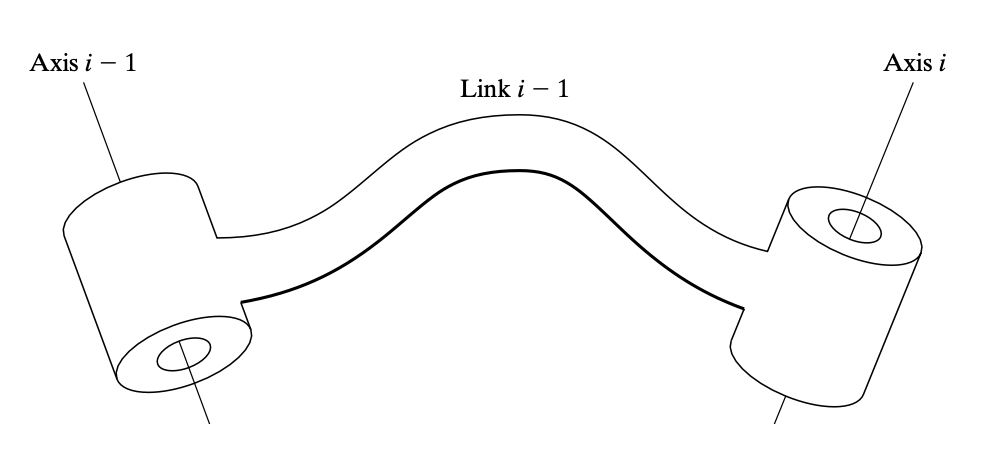
\includegraphics[width=.5\textwidth]{forward-kinematics/kinematic-chain.png}
\end{figure}

\subsection{Articulations and joint speed}
\subsubsection{Joint types and degrees of freedom}
The topology of the articulation between two rigid bodies defines the degrees of freedom of the joint.
\begin{figure}[H]
    \centering
    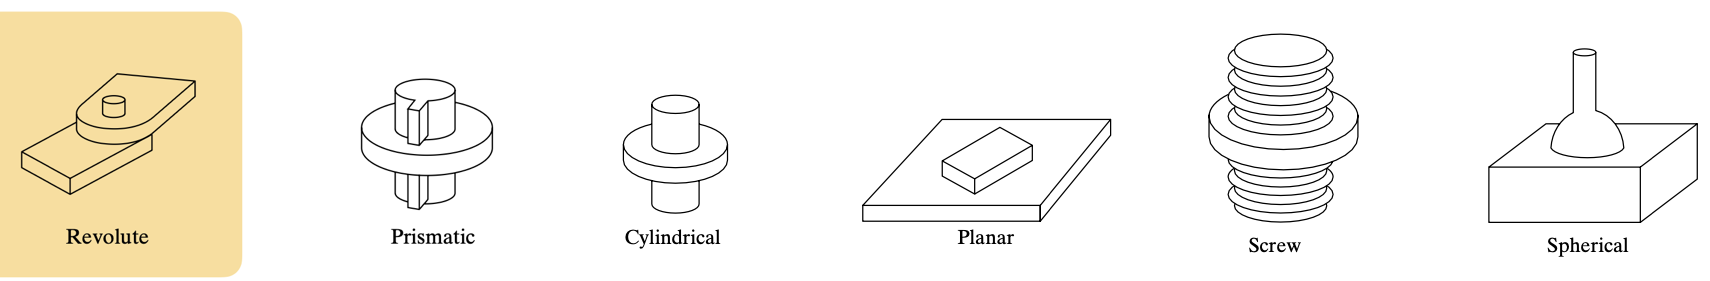
\includegraphics[width=.9\textwidth]{forward-kinematics/joints.png}
    \caption{Example of possible joints.}
\end{figure}
Each joint can be represented as a function $K_i$ from a configuration space $Q_i$ to the Special Euclidean Group $\SE(3)$:
\begin{equation*}
    \begin{aligned}
        K_i: Q_i &\longrightarrow \SE(3)\\
        q &\longmapsto M_i(q_i)
    \end{aligned}
\end{equation*}

Consider for instance the revolute joint, which constrains the motion of two bodies around a fixed axis. It is parameterized by the angle $\theta\in\R$, therefore the configuration space is $Q_i=\Sb^1\simeq\R$ (one degree of freedom). The function $K_i$ is then defined as:
\begin{equation*}
    \begin{aligned}
        K_i: \Sb^1\simeq\R &\longrightarrow \SE(3)\\
        q &\longmapsto \begin{bmatrix}
            \cos  & -\sin q & 0 & 0\\
            \sin q & \phantom{-}\cos q & 0 & 0\\
            0 & 0 & 1 & 0\\
            0 & 0 & 0 & 1
        \end{bmatrix}
    \end{aligned}
\end{equation*}

\subsubsection{Joint speed}
The change of configuration of the joint comes from the joint speed, which is the derivative of the joint parameter with respect to time. Consider the relative position of the articulation between the two adjactent frames, given by:
\begin{equation*}
    \begin{aligned}
        K_i : Q_i &\longrightarrow \SE(3)\\
        q_i &\longmapsto M_i(q_i)
    \end{aligned}
\end{equation*}
The relative speed of the joint generated by the articulation is given by:
\begin{equation*}
    \begin{aligned}
        k_i:T_{q_i}Q_i &\longrightarrow \se(3)\\
        (q_i, \dot{q}_i) &\longmapsto v_i(q_i) = S_i(q_i)\dot{q}_i
    \end{aligned}
\end{equation*}
for some transformation $S_i$.

In the case of the revolute joint, the speed of the joint is given by:
\begin{equation*}
    \begin{aligned}
        k_i: T_q\Sb^1\simeq\R^2 &\longrightarrow \se(3)\\
        (q, \dot{q}) &\longmapsto (v, w) = \left(
            \begin{bmatrix}
                0\\0\\0
            \end{bmatrix}, \begin{bmatrix}
                0\\0\\\dot{q}
            \end{bmatrix}\right)
    \end{aligned}
\end{equation*}
Hence, we have:
\begin{equation*}
    S_i(q) = \begin{bmatrix}
        0\\0\\0\\0\\0\\1
    \end{bmatrix} \in \mathscr{M}_{6, 1}(\R)
\end{equation*}
which gives us $S_i(q)\dot{q}=(v,w)$ as expected.

\subsection{Direct geometry}
We aim to compute the position and orientation of the terminal organ given the joint parameters. We can do so by computing the transformation matrix of each body in the kinematic chain, and then multiplying them to get the transformation matrix of the terminal organ.

\subsubsection{Transformation matrix}
Given an articulation $i$, we can compute the relative position of the associated frame $i$ with respect to the frame $i-1$ using the function $K_i$:
\begin{equation*}
    \prescript{i-1}{}{M_i(q_i)} = \prescript{i-1}{}{P_iK_i(q_i)}
\end{equation*}
We can combine the transformations of all the bodies in the kinematic chain to get the transformation matrix of the terminal organ:
\begin{equation*}
    \begin{aligned}
        \prescript{0}{}{K_n} : \bigtimes_{i=1}^n Q_i &\longrightarrow \SE(3)\\
        q=(q_1, \dots, q_n) &\longmapsto \bigtimes_{i=1}^n \prescript{i-1}{}{M_i(q_i)}
    \end{aligned}
\end{equation*}
Therefore, the configuration space can be read as the product of the configuration spaces of each joint:
\begin{equation*}
    Q = \bigtimes_{i=1}^N Q_i \simeq \R^{\sum_{i=1}^N n_i}
\end{equation*}
where $N$ is the number of joints.

\subsubsection{Kinematic Jacobian}
Our goal is now to link the joint speed to the spatial speed of the bodies in movement. For each articulation, we have a linear mapping of the form:
\begin{equation*}
    v_i(q_i) = S_i(q_i)\dot{q_i}
\end{equation*}
This corresponds to the temporal derivative of the articular geometry:
\begin{equation*}
    \dot{M}_i(q_i)M_i^{-1}(q_i) = S_i(q_i)\dot{q}_i
\end{equation*}
Therefore, one can link the spatial speed of a body to the joint speed using the relation:
\begin{equation*}
    \prescript{0}{}{k_n}(q, \dot{q}) = \sum_{i=1}^n k_i(q_i, \dot{q}_i) = \underbrace{\begin{bmatrix}
        S_1(q_1) \cdots S_n(q_n)
    \end{bmatrix}}_{J(q)}
    \begin{bmatrix}
        \dot{q}_1\\\vdots\\\dot{q}_n
    \end{bmatrix}
\end{equation*}
\section{Inverse Kinematics}
\emph{Inverse Kinematics} aims at finding joint parameters that achieve a desired end-effector pose. This is a more complex problem than forward kinematics, as it is not always possible to find a solution, and when it is, there may be multiple solutions.
\begin{figure}[H]
    \centering
    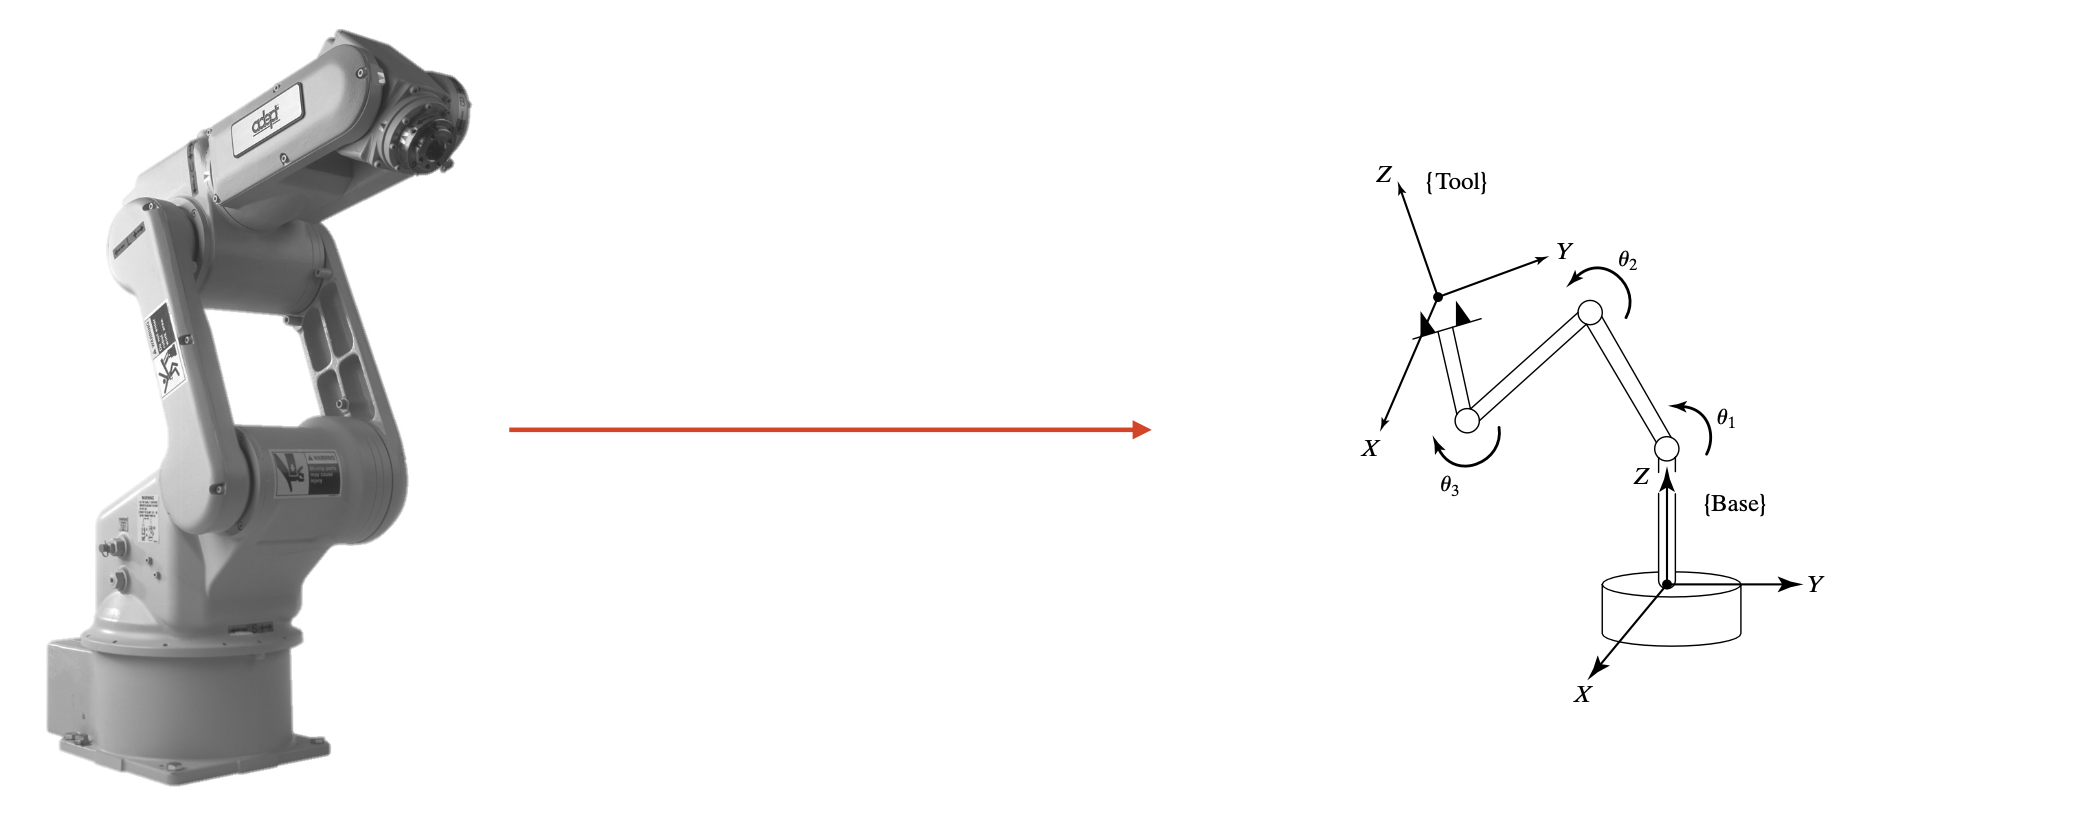
\includegraphics[width=0.8\textwidth]{inverse-kinematics/inverse-kinematics.png}
\end{figure}

\subsection{Optimization problem and resolution}
Given a target position $M^*$ for the end-effector, we aim at solving the following distance minimization problem:
\begin{equation*}
    \min_{q\in Q} d(\prescript{0}{}{K_n(q)}, M^*)
\end{equation*}
Using the logarithm distance, we can rewrite the problem as:
\begin{equation}
    \min_{q\in Q} \norm{\log(\prescript{0}{}{K_n(q)}^{-1}M^*)}
\end{equation}
We can cast this initial problem $\min_{q\in Q} \norm{\log(\prescript{0}{}{K_n(q)}^{-1}M^*)}$ as a more general optimization problem:
\begin{equation*}
    \min_{x\in\R^n}\frac{1}{2}\norm{f(x)}_2^2
\end{equation*}
We aim at iteratively solving this optimization problem. A first-order linear approximation of $f$ around $x$ is given by:
\begin{equation*}
    f(x+p)=f(x)+\underbrace{\partfrac{f}{x}(x)}_{J(x)}p
\end{equation*}
Hence:
\begin{equation*}
    \min_{p\in\R^n}\frac{1}{2}\norm{f(x_0+p)}_2^2 = \min_{p\in\R^n}\frac{1}{2}\norm{f(x)+J(x)p}_2^2
\end{equation*}
We can now solve the optimization problem by setting the gradient of the objective function to zero:
\begin{equation*}
    \begin{aligned}
        &\nabla_p\left(\frac{1}{2}\norm{f(x)+J(x)p^*}_2^2\right)=0\\
        \iff &J(x)^\tp (f(x)+J(x)p^*) = 0\\
        \iff &p^* = -(J(x)^\tp J(x))^{-1}J(x) f(x)\\
        \iff &p^* = -J(x)^+ f(x)
    \end{aligned}
\end{equation*}
where $J(x)^+$ is the \emph{Moore-Penrose pseudoinverse} of $J(x)$. We can then iteratively update:
\begin{equation*}
    x_{k+1} = x_k + \alpha p_k
\end{equation*}
until we obtain $\norm{J(x)^\tp f(x)}\leq\epsilon^*$, where $\epsilon^*>0$ is a fixed precision we aim at achieving. This iterative method is known as the \emph{Newton-Raphson} method. If we work on a differential manifold, we can use instead:
\begin{equation*}
    q_{k+1}=q_l\oplus\alpha p_k
\end{equation*}

\subsection{Trajectory tracking}
We can extend the previous method to track a trajectory $M(t)$: we want to compute the joint speeds $\dot{q}$ that track the trajectory as closely as possible. Consider a continuous and differentiable time trajectory $M^*$:
\begin{equation*}
    \begin{aligned}
        M^*:[0, T]&\longrightarrow \SE(3)\\
        t&\longmapsto M^*(t)
    \end{aligned}
\end{equation*}
We are also given the corresponding spatial (linear and angular) velocity of the end-effector $v^*$:
\begin{equation*}
    \begin{aligned}
        v^*:[0, T]&\longrightarrow\se(3)\\
        t&\longmapsto v^*(t)
    \end{aligned}
\end{equation*}

At each instant $t$, the forward kinematics of the robot give us the current end-effector pose $M(t)$ and the corresponding Jacobian $J(t)$:
\begin{equation*}
    M(q(t)) = \bigtimes_{i=0}^n K_i(q_i(t)) \in\SE(3)
    \quad\text{and}\quad
    v(t) = J(q(t))\dot{q}(t)\in\se(3)
\end{equation*}
Using the angular speed of the joints $\dot{q}(t)$, we can control the position $q(t)$ of the joints. Our goal is to minimize the gap between the position and speed of the end-effector $(M(q(t)), v(q(t), \dot{q}(t)))$ and the desired trajectory $(M^*(t), v^*(t))$.

The error can be computed using the following cost function:
\begin{equation*}
    e(t, q(t)) = M(q(t)) \ominus M^*(t) = \log_{\SE(3)}\left(M^*(t)^{-1}M(q(t))\right)
\end{equation*}
The error in velocity space is given by:
\begin{equation*}
    \dot{e}(t, q(t), \dot{q}(t)) = v(q(t), \dot{q}(t)) - v^*(t) = J(q(t))\dot{q}(t) - v^*(t)
\end{equation*}
We define the error correction profile as:
\begin{equation*}
    \dot{e}(t, q(t), \dot{q}(t)) = -\lambda e(t, q(t))
\end{equation*}
for some $\lambda>0$. This finally gives us the following optimization problem:
\begin{equation}
    \boxed{\min_{\dot{q}(t)} \frac{1}{2}\norm{\dot{e}+\lambda e}_2^2}
\end{equation}
\section{Motion planning}
\subsection{Configuration space}

\section{Collision Detection}
Collision detection is a subject at the center of physics simulators. To build a simulation of the robot in its environment, the main loop goes as follows:
\begin{enumerate}
    \item Collision detection: finding contact points
    \item Collision resolution: finding contact forces using physical principles
    \item Time integration: update of the quantities of interest (position, velocity, etc.)
\end{enumerate}
It is therefore crucial to have an efficient collision detection algorithm, that is to know whether two objects are in contact or not, and if so, to find the contact points.

Nevertheless, collision detection is a computational bottleneck in physics simulators. Resolving collision detection for one pair of objects takes a significant amount of time, especially for complex shapes, and the number of pairs to check grows quadratically with the number of objects. A general method to optimize such a process is to decompose one collision detection into two phases, the broad phase and the narrow phase. The broad phase uses simple geometric primitives to quickly discard pairs of objects that are far from colliding. The narrow phase then uses more complex geometric primitives to find the exact contact points.

\subsection{The broad phase}

\subsection{The narrow phase}

\newpage
% \section{Reinforcement Learning}
% \section{Locomotion}

\end{document}